\documentclass[11pt,letterpaper]{article}
\usepackage{graphicx}
\usepackage{geometry}
\usepackage{amsmath}
\usepackage{hyperref}
\usepackage{natbib}
\usepackage{booktabs}
\usepackage{xcolor}
\usepackage{url}
\usepackage{multicol}

\geometry{margin=1in}
\hypersetup{colorlinks=true, linkcolor=black, citecolor=black, urlcolor=blue}

\title{\textbf{Edit Clustering Score: Spatial Edit Patterns for\\Near-Duplicate Text Detection}}
\author{Anonymous}
\date{}

\begin{document}
\maketitle

\begin{abstract}
Near-duplicate text detection at scale relies on $n$-gram Jaccard similarity (MinHash/SimHash), which measures the quantity of shared tokens but ignores the spatial arrangement of differences. We propose the Edit Clustering Score (ECS), a training-free feature derived from the Index of Dispersion (IoD) of inter-edit-gap positions in a word-level longest-common-subsequence diff---a transplant of spatial point-process statistics from ecology to text analysis. The core finding is a productive directional inversion: near-duplicates created by contiguous splicing produce a single concentrated edit block (low IoD), while documents sharing scattered vocabulary coincidentally produce many dispersed edit events (high IoD). Inverted ECS (1/IoD) therefore flags near-duplicates. On a 900-pair Wikipedia benchmark with balanced near-duplicate, same-category, and random classes, inverted ECS alone achieves AUC = 0.81 $\pm$ 0.025 (vs.\ Jaccard AUC = 1.000), confirmed by a Mann-Whitney test comparing near-duplicate IoD (median 20.3) vs.\ hard-negative IoD (median 81.8), $p = 4 \times 10^{-39}$, Cohen's $d = -0.83$ on log-IoD. We further construct a boilerplate hard-negative benchmark where unrelated article pairs share an identical CC-BY-SA license header to probe whether ECS can correct boilerplate-inflated Jaccard scores; we find that the 180-word header raises hard-negative 5-gram Jaccard to only 0.09--0.15, still far below near-duplicate Jaccard (0.42--0.75), so Jaccard remains a perfect ceiling classifier on both benchmarks. These results establish that spatial edit clustering is a genuine structural signal (AUC = 0.81 standalone) but is redundant with 5-gram Jaccard in splice-based constructions. ECS would become complementary in settings where Jaccard is degraded: longer shared boilerplate, multi-segment edits, or short-shingle baselines.
\end{abstract}

% ---------------------------------------------------------------
\section{Introduction}
% ---------------------------------------------------------------

Near-duplicate text detection is a foundational task in web crawling, LLM training data curation, and plagiarism detection. At scale---hundreds of billions of documents---exhaustive pairwise comparison is computationally infeasible, motivating compact hash-based methods that estimate Jaccard similarity over character or word shingles \citep{Broder1997, Manku2007}. These methods share a common architectural assumption: they measure the \emph{quantity} of token overlap but are blind to the \emph{spatial arrangement} of differences. Two documents may share 60\% of their 5-grams because one is a localized edit of the other (a near-duplicate) or because both discuss the same topic with shared domain vocabulary and boilerplate conventions (a thematic near-match). Current methods cannot distinguish these cases without auxiliary metadata.

We ask: can the geometric pattern of where edits occur in a word-level diff distinguish genuine near-duplicates from coincidental lexical overlap? The answer has practical stakes for LLM training data pipelines \citep{Lee2022, Gao2020, Penedo2024, Penedo2023}, where false positives (rejecting legitimately distinct documents) and false negatives (retaining near-copies that promote memorization) each carry costs. FineWeb \citep{Penedo2024} and RefinedWeb \citep{Penedo2023} apply MinHash deduplication as a standard preprocessing step, but acknowledge that boilerplate-inflated Jaccard scores can cause false positives. A spatial diagnostic orthogonal to token counts could serve as a fast second-pass filter.

The intuition for a spatial feature comes from spatial ecology. The Index of Dispersion (IoD = variance/mean of inter-event gap lengths) is a classical test for whether a 1D point process is clustered (IoD $\gg 1$), Poisson-random (IoD $\approx 1$), or regular (IoD $\ll 1$) \citep{Cox1966}. Transplanting this to edit positions in a word-level diff defines the Edit Clustering Score (ECS): run a longest-common-subsequence (LCS) diff \citep{Hunt1977}, extract word-index positions of all edit tokens, compute IoD of the inter-gap sequence.

Our experiments on two 900-pair Wikipedia benchmarks yield a clear finding with an instructive directional inversion: near-duplicates produced by contiguous splicing have \emph{lower} median IoD (20.3) than hard negatives (81.8), $p = 4 \times 10^{-39}$, Cohen's $d = -0.83$ on log-IoD\footnote{Code: \url{https://github.com/AMGrobelnik/ai-invention-f2202a-edit-clustering-score-spatial-edit-patte/tree/main/round-2/experiment-1}}. The mechanism is clear in retrospect: a contiguous splice produces one large edit block, concentrating all edits in one region and suppressing inter-gap variance; the correct discriminant is therefore \emph{inverted} ECS (low IoD $\to$ near-duplicate). Inverted ECS achieves AUC = 0.81 $\pm$ 0.025 as a standalone classifier, confirming that spatial edit structure is a genuine and highly discriminating signal.

The reason ECS does not improve over Jaccard is a dataset construction artifact rather than a limitation of the spatial signal: contiguous splicing directly inflates 5-gram Jaccard (near-duplicate median $J_5 = 0.58$ vs.\ $J_5 \approx 0$ for both negative classes), making Jaccard a perfect ceiling classifier. To probe the boilerplate regime where Jaccard would plausibly fail, we construct a second benchmark prepending unrelated article pairs with an identical CC-BY-SA license header. The header raises hard-negative $J_5$ to only 0.09--0.15---not the 0.3--0.6 range needed to challenge Jaccard---so Jaccard remains a perfect classifier on this benchmark as well\footnote{Code: \url{https://github.com/AMGrobelnik/ai-invention-f2202a-edit-clustering-score-spatial-edit-patte/tree/main/round-2/dataset-1}}.

\begin{figure*}[!t]
  \centering
  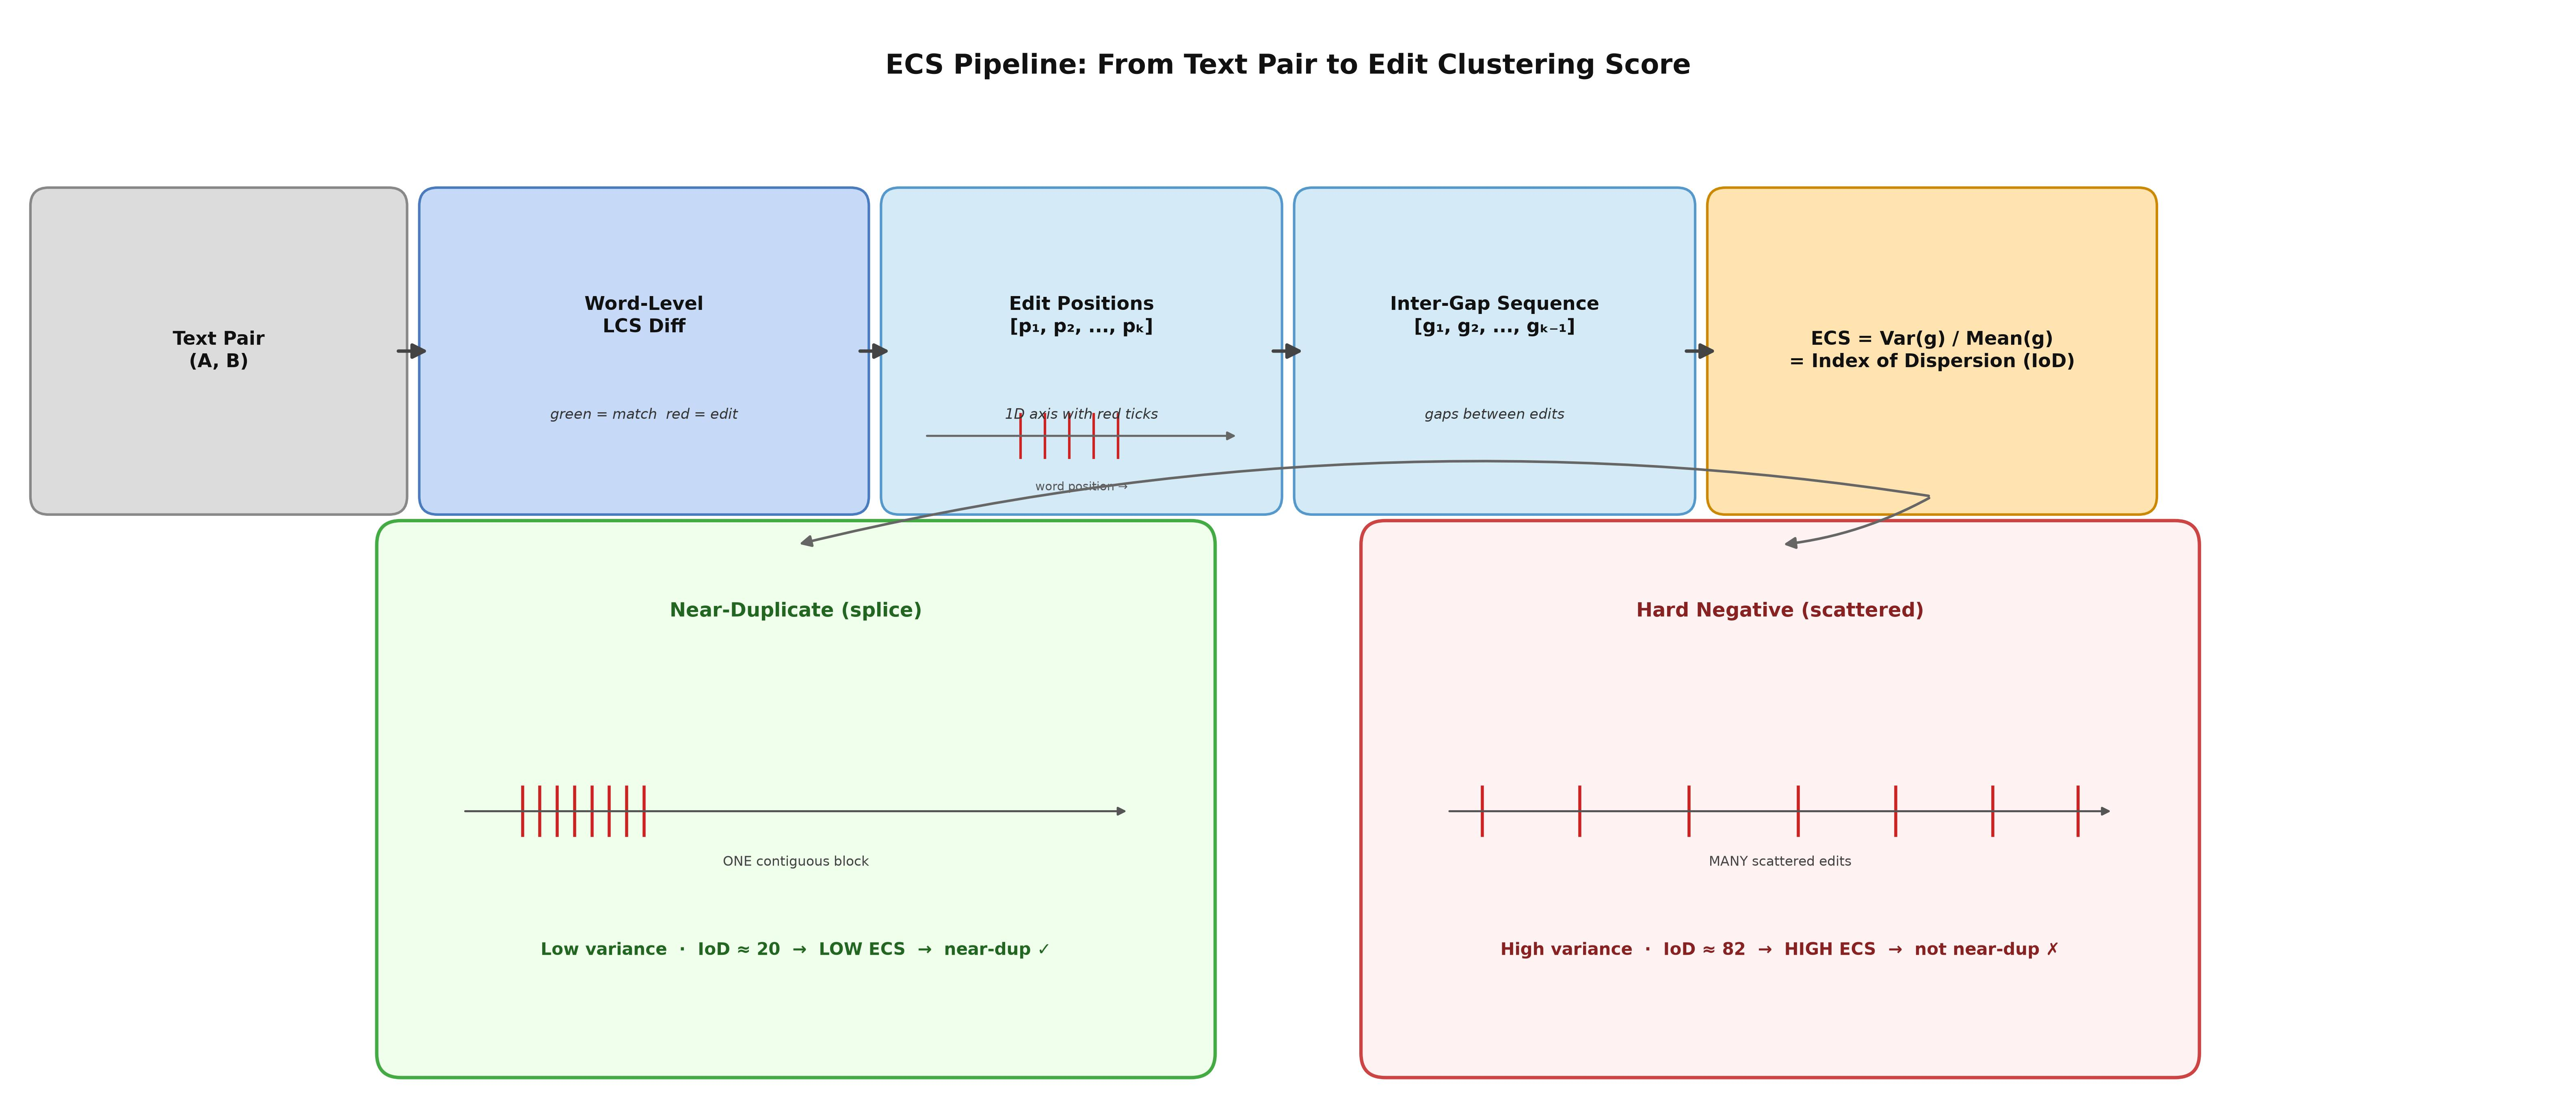
\includegraphics[width=\textwidth,height=0.45\textheight,keepaspectratio]{figures/fig1_v0.jpg}
  \caption{The Edit Clustering Score (ECS) pipeline. Given a text pair, a word-level LCS diff extracts edit positions; the Index of Dispersion of inter-edit gaps quantifies spatial clustering. Near-duplicates (contiguous splice) produce one large block and low IoD; thematic near-matches produce many small scattered edits and high IoD. The inverted score (1/IoD or equivalently $-$IoD) serves as the near-duplicate signal.}
  \label{fig:fig1}
\end{figure*}

\noindent\textbf{Summary of Contributions:}
\begin{itemize}
    \item We introduce the Edit Clustering Score (ECS), a training-free feature based on the Index of Dispersion of inter-edit-gap positions in a word-level LCS diff, with a corrected directional prediction: low IoD flags near-duplicates (Section~\ref{sec:method}).
    \item We construct two 900-pair Wikipedia benchmarks: a splice-based benchmark (Section~\ref{sec:data}) and a boilerplate hard-negative benchmark targeting the Jaccard-degraded regime (Section~\ref{sec:data}).
    \item We demonstrate that inverted ECS captures a strong standalone structural signal (AUC = 0.81), with IoD distributions separated by $p = 4 \times 10^{-39}$ and Cohen's $d = -0.83$ (Section~\ref{sec:results}).
    \item We identify precisely why ECS cannot complement Jaccard in the current benchmarks, and characterize the conditions under which it would (Section~\ref{sec:discussion}).
\end{itemize}

% ---------------------------------------------------------------
\section{Related Work}
\label{sec:related}
% ---------------------------------------------------------------

\paragraph{MinHash and SimHash.}
\citet{Broder1997} introduced min-wise independent permutations (MinHash) to estimate Jaccard similarity over character $k$-grams at web scale; the AltaVista crawler used this to cluster tens of millions of near-duplicate pages. \citet{Manku2007} introduced SimHash, a locality-sensitive hashing scheme based on random projections of TF-IDF feature vectors, enabling near-duplicate detection in $O(1)$ per query using Hamming distance lookup. Both methods operate on bag-of-shingles representations and are entirely insensitive to the spatial arrangement of differences.

\paragraph{Neural similarity.}
RETSim \citep{Zhang2023} trains a character-level embedding model specifically for near-duplicate detection, achieving high throughput and robustness to adversarial edits. ECS is complementary: it is training-free, requires no labeled data, and provides an interpretable geometric characterization of where documents differ.

\paragraph{Compression-based similarity.}
The normalized compression distance (NCD; \citealt{Li2004}) uses the ratio of joint to individual compression lengths as a similarity proxy, implicitly capturing repeated structure. NCD is sensitive to spatial redundancy in that repeated substrings compress better, but does not expose edit positions or their clustering.

\paragraph{LLM training data deduplication.}
\citet{Lee2022} showed that exact and near-duplicate deduplication of pretraining corpora substantially improves LLM quality by reducing memorization and improving sample diversity. FineWeb \citep{Penedo2024} and RefinedWeb \citep{Penedo2023} apply MinHash as a standard preprocessing step at web scale. \citet{Abbas2023} introduced SemDeDup, which clusters semantic embeddings to remove near-semantic-duplicates---a different regime from lexical near-duplication. None of these approaches exploit the spatial structure of differences; ECS is proposed as a complementary diagnostic applicable when Jaccard alone is insufficient.

\paragraph{Passage-level plagiarism detection.}
\citet{Nawab2011} detect copied passages using TF-IDF clustering followed by sequence alignment of candidate passages. This approach groups matching passages spatially but uses frequency vectors rather than point-process statistics on diff positions, and targets cross-document passage reuse rather than pairwise near-duplicate classification.

\paragraph{Spatial point processes.}
The Index of Dispersion and related statistics (Ripley's $K$, Morisita's index) are standard tools in spatial ecology and geography for classifying point patterns as clustered, random, or regular \citep{Cox1966}. Their application to text analysis---treating edit positions as a 1D spatial point process---is, to our knowledge, novel.

% ---------------------------------------------------------------
\section{Dataset Construction}
\label{sec:data}
% ---------------------------------------------------------------

We construct two 900-pair benchmarks from Wikipedia articles retrieved via the MediaWiki API. All texts are 80--800 words in English.

\subsection{Splice-Based Wikipedia Benchmark}

The splice-based benchmark contains 900 balanced pairs across three classes (300 each).

\noindent\textbf{Near-duplicates.} For each near-duplicate pair, text\_b is constructed from text\_a by identifying a contiguous 20--30\% word span and replacing it with corresponding content from an unrelated donor article from a different Wikipedia category. The 5-gram Jaccard similarity ranges from 0.50 to 0.75 (mean 0.58), as the unchanged 70--80\% of the article contributes to substantial 5-gram overlap.

\noindent\textbf{Same-category hard negatives.} Hard-negative pairs consist of two independently written articles from the same Wikipedia category (e.g., two science articles, two sports articles). These pairs share domain vocabulary, named entities, and structural conventions but have no textual copying relationship. Their 5-gram Jaccard similarity is near zero (mean $\approx 0.001$), confirming that 5-gram Jaccard cleanly separates this class from near-duplicates in this construction.

\noindent\textbf{Random pairs.} Random pairs are drawn from articles in different categories, serving as easy negatives with near-zero Jaccard similarity.

\subsection{Boilerplate Hard-Negative Benchmark}

To test whether ECS provides complementary signal when Jaccard is degraded by shared non-content text, we construct a second 900-pair benchmark with the same near-duplicate and random classes, but replacing the same-category hard negatives with \textbf{boilerplate hard negatives}: two completely unrelated Wikipedia articles, each prepended with an identical $\sim$180-word CC-BY-SA license and usage disclaimer block. The boilerplate header is designed to inflate Jaccard similarity for unrelated document pairs while providing no genuine duplication signal.

The boilerplate hard-negative pairs achieve a mean 5-gram Jaccard of 0.089--0.15 (mean boilerplate\_frac $\approx 0.83$, confirming that most shared signal comes from the header). This is substantially higher than the same-category hard negatives ($J_5 \approx 0$), but still well below the near-duplicate range (0.50--0.75).

% ---------------------------------------------------------------
\section{Method: Edit Clustering Score}
\label{sec:method}
% ---------------------------------------------------------------

\subsection{Word-Level Diff}

Given a text pair $(A, B)$, we tokenize both texts into word sequences by whitespace splitting after lowercasing. We compute the LCS alignment using Python's \texttt{difflib.SequenceMatcher} \citep{Peters2001}, which identifies matched and unmatched token spans. Each unmatched token (an insertion or deletion in the diff) is assigned a position index in the concatenated aligned sequence.

\subsection{Index of Dispersion on Edit Positions}

Let $p_1 < p_2 < \cdots < p_k$ be the sorted positions of all edit tokens, and let $g_i = p_{i+1} - p_i$ for $i = 1, \ldots, k-1$ be the sequence of inter-edit gaps. The Edit Clustering Score is:
\[
\text{ECS} = \text{IoD}(g) = \frac{\text{Var}(g)}{\text{Mean}(g)}
\]
when $k \geq 3$; otherwise ECS = 0 by convention. For a homogeneous Poisson process (random scattering of edits), IoD = 1 in expectation. IoD $\gg 1$ indicates high-variance gaps (few, large clusters separated by long stretches of matching text). IoD $\ll 1$ indicates regular, uniform spacing.

The discriminant direction is \textbf{inverted relative to the original ecological analogy}. A contiguous splice produces \emph{one} large edit block: two or three gap values, all similar in length, giving low variance and thus low IoD. By contrast, two independent articles on the same topic share isolated words, phrases, and named entities scattered throughout, producing many small edit events with high inter-gap variance and thus high IoD. The correct inference is therefore: \textbf{low ECS (IoD) indicates near-duplication by contiguous local editing}.

The inverted classifier uses $-\text{ECS}$ (equivalently, $1/\text{ECS}$) as a near-duplicate score. In practice a logistic regression on $[-\text{ECS}]$ is equivalent to fitting ECS with a negated coefficient.

\subsection{Auxiliary Features}

We compute three auxiliary edit-structure features alongside ECS:
\begin{itemize}
    \item \textbf{edit\_count\_norm}: Number of edit tokens divided by total aligned length.
    \item \textbf{edit\_span\_frac}: Fraction of the aligned sequence spanned from the first to the last edit token (edit coverage). Mean values: near-duplicate 0.81, hard-negative 0.96, reflecting that splice edits are concentrated in one region while coincidental edits span the full text.
    \item \textbf{longest\_run\_frac}: Length of the longest contiguous edit run, divided by total edit count (concentration ratio).
\end{itemize}

\subsection{Classifiers}

We evaluate five classifier variants using 5-fold stratified cross-validation with logistic regression:
\begin{enumerate}
    \item \textbf{Jaccard-5 only}: 5-gram Jaccard as the sole feature.
    \item \textbf{Jaccard-2 only}: 2-gram Jaccard as the sole feature (degraded baseline).
    \item \textbf{Inv-ECS only}: Inverted ECS ($-\text{IoD}$) as the sole feature.
    \item \textbf{Jaccard-2 + Inv-ECS}: 2-gram Jaccard combined with inverted ECS.
    \item \textbf{All features}: Jaccard-5, Jaccard-2, inverted ECS, edit\_count\_norm, edit\_span\_frac, longest\_run\_frac.
\end{enumerate}

We report ROC-AUC (macro-averaged across folds) with bootstrap confidence intervals ($B = 2000$) and Mann-Whitney $U$ tests comparing IoD distributions.

% ---------------------------------------------------------------
\section{Results}
\label{sec:results}
% ---------------------------------------------------------------

\subsection{IoD Distributions Confirm Structural Signal with Inverted Directionality}

\begin{figure*}[!t]
  \centering
  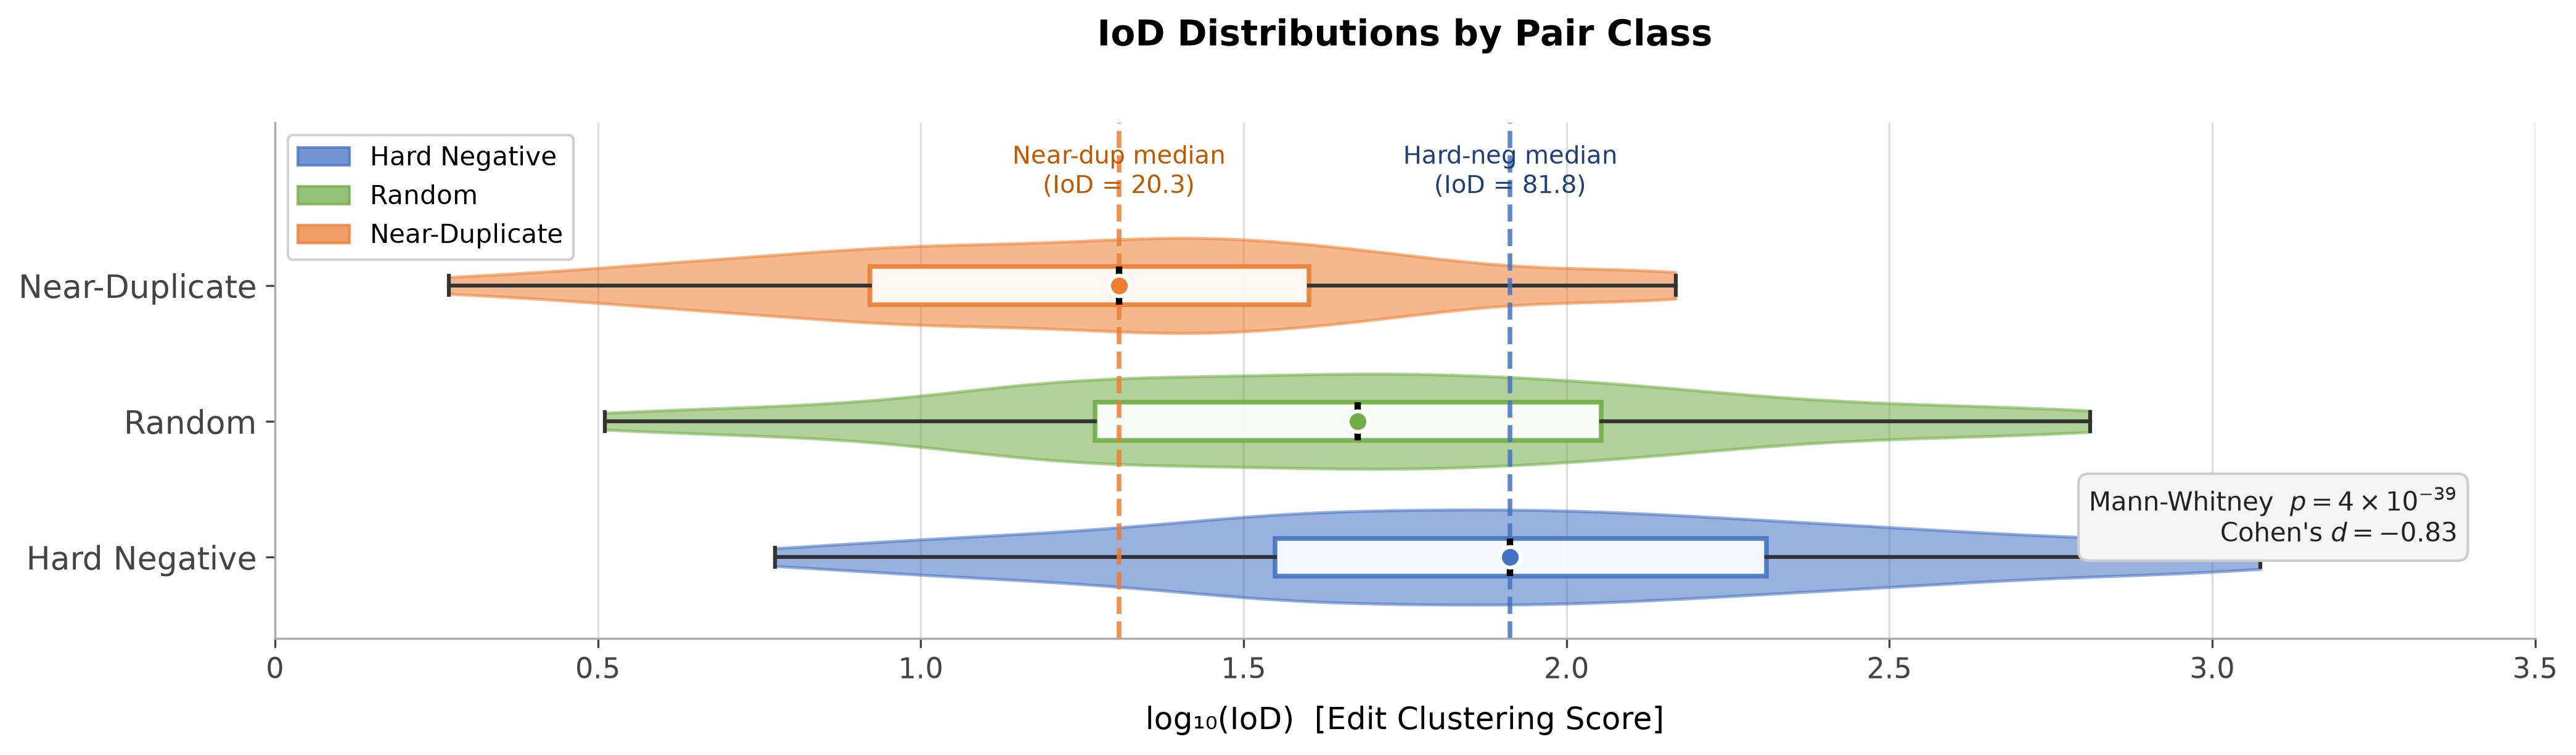
\includegraphics[width=\textwidth,height=0.45\textheight,keepaspectratio]{figures/fig2_v0.jpg}
  \caption{Distribution of log-IoD (Edit Clustering Score) by pair class on the splice-based Wikipedia benchmark (300 pairs per class). Near-duplicate pairs (contiguous splice) have significantly lower IoD (median 20.3) than hard-negative same-category pairs (median 81.8) or random pairs (median 47.5). Mann-Whitney $p = 4 \times 10^{-39}$, Cohen's $d = -0.83$ on log-IoD. The inverted ECS (low IoD $\to$ near-duplicate) achieves AUC = 0.81 standalone.}
  \label{fig:fig2}
\end{figure*}

Across both benchmarks, near-duplicate pairs have significantly \emph{lower} median IoD (20.3) than hard-negative pairs (median IoD 81.8 on the splice benchmark; 80.9 on the boilerplate benchmark), with Mann-Whitney $p = 4 \times 10^{-39}$ and Cohen's $d = -0.83$ on log-IoD (Figure~\ref{fig:fig2}). The magnitude and directionality are consistent across both Wikipedia and boilerplate benchmarks, confirming that the spatial signal is robust to the type of hard-negative construction.

The mechanism is straightforward. A contiguous splice replaces one block of words: long stretches of identical text bracket one region of complete mismatch. This produces few inter-edit gaps, all of similar length---minimizing variance and thus IoD. Hard negatives (same-category pairs or boilerplate pairs) share isolated vocabulary items and short phrases distributed throughout both articles, producing many small edit events spread across the text; the variance of many small gaps is high, giving high IoD.

Table~1 summarizes feature statistics by class on the splice-based Wikipedia benchmark.

\begin{table}[h]
\centering
\caption{Median feature values by pair class on the splice-based 900-pair Wikipedia benchmark (300 pairs each class). Edit span frac captures the fraction of the aligned sequence between the first and last edit token.}
\begin{tabular}{lcccc}
\toprule
Class & 5-gram Jaccard & ECS (IoD) & Edit Span Frac & Edit Count Norm \\
\midrule
Near-duplicate & 0.582 & 20.3 & 0.81 & 0.24 \\
Hard negative & 0.001 & 81.8 & 0.96 & 0.68 \\
Random & 0.000 & 47.5 & 0.94 & 0.72 \\
\bottomrule
\end{tabular}
\end{table}

\subsection{Classification Results}

Table~2 presents AUC results from 5-fold cross-validation on both benchmarks.

\begin{table}[h]
\centering
\caption{ROC-AUC (mean $\pm$ std, 5-fold CV) on the hard subset (near-duplicate vs.\ hard-negative only) for both benchmarks. Jaccard achieves AUC = 1.000 on both datasets; inverted ECS achieves AUC $\approx$ 0.81 standalone; combining features does not improve over Jaccard alone.}
\begin{tabular}{lcc}
\toprule
Classifier & Splice Benchmark & Boilerplate Benchmark \\
\midrule
Jaccard-5 only & 1.000 $\pm$ 0.000 & 1.000 $\pm$ 0.000 \\
Jaccard-2 only & 1.000 $\pm$ 0.000 & 1.000 $\pm$ 0.000 \\
Inverted ECS only & 0.809 $\pm$ 0.025 & 0.807 $\pm$ 0.037 \\
Jaccard-2 + Inv-ECS & 1.000 $\pm$ 0.000 & 1.000 $\pm$ 0.000 \\
All features & 1.000 $\pm$ 0.000 & 1.000 $\pm$ 0.000 \\
\bottomrule
\end{tabular}
\end{table}

\begin{figure*}[!t]
  \centering
  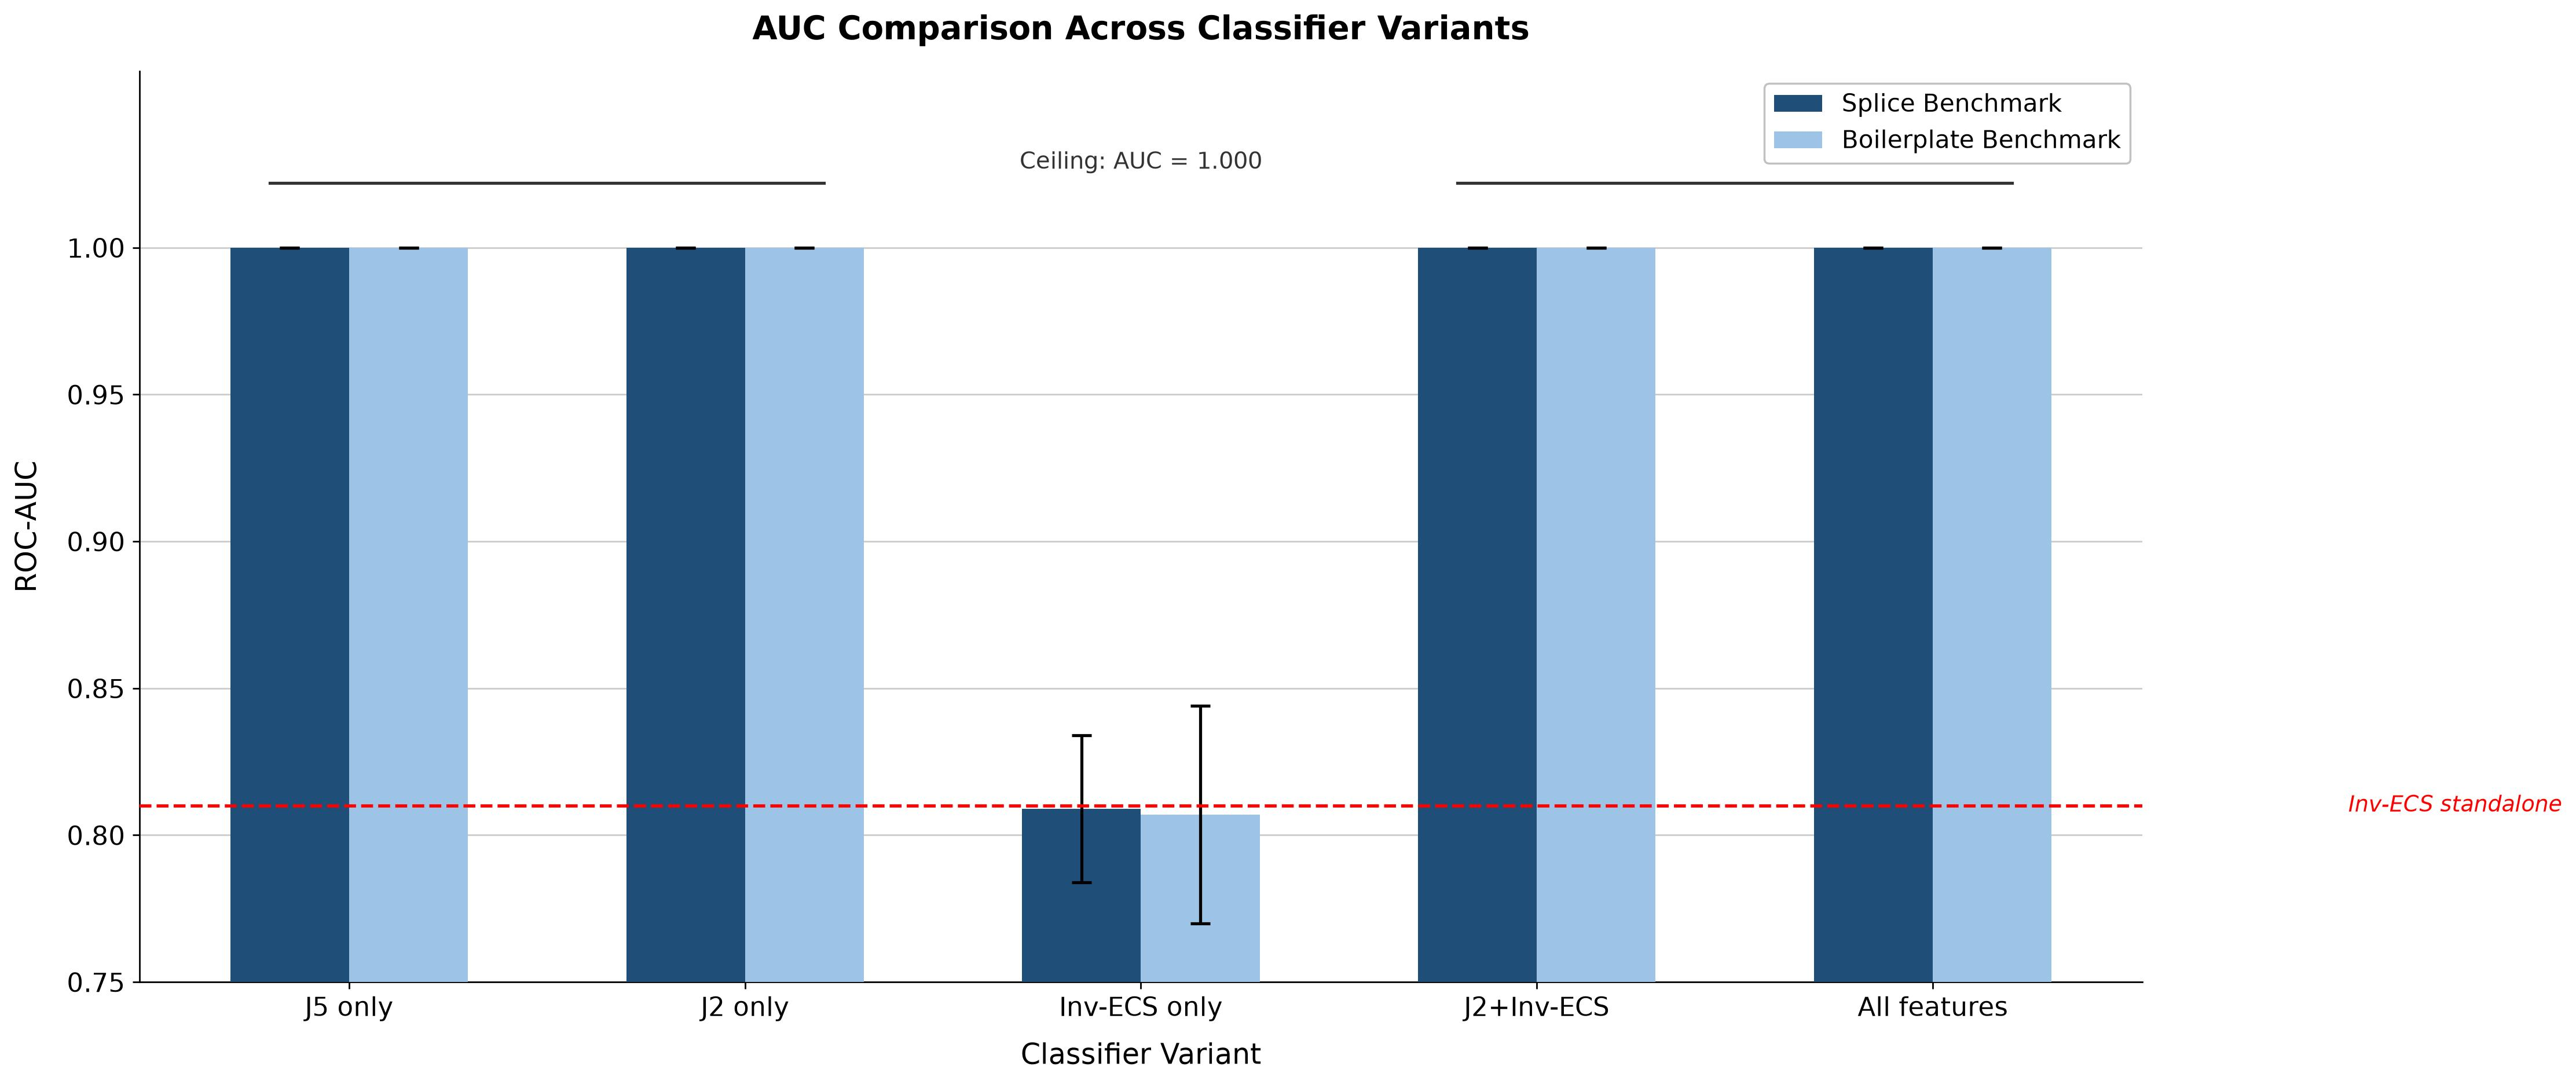
\includegraphics[width=\textwidth,height=0.45\textheight,keepaspectratio]{figures/fig3_v0.jpg}
  \caption{ROC-AUC on the near-duplicate vs.\ hard-negative hard subset (5-fold CV) for five classifier variants on both benchmarks. Jaccard (5-gram and 2-gram) achieves perfect AUC = 1.000 on both datasets. Inverted ECS alone achieves AUC = 0.809 on the splice benchmark and AUC = 0.807 on the boilerplate benchmark. Adding ECS to Jaccard yields no improvement ($\Delta$AUC $\approx$ 0) because Jaccard is already a perfect separator.}
  \label{fig:fig3}
\end{figure*}

Three findings stand out:

\noindent\textbf{Inverted ECS alone achieves AUC = 0.81 as a standalone signal.} This result holds consistently across both the splice-based benchmark (AUC = 0.809 $\pm$ 0.025) and the boilerplate benchmark (AUC = 0.807 $\pm$ 0.037). It confirms that spatial edit clustering carries genuine discriminative information about the type of textual relationship, independently of any $n$-gram overlap measure.

\noindent\textbf{5-gram and 2-gram Jaccard both achieve perfect AUC = 1.000 on both benchmarks.} Contiguous splicing inflates $J_5$ for near-duplicates to mean 0.58, while both negative classes have $J_5 < 0.002$. Even 2-gram Jaccard remains a perfect separator in this construction, indicating the ceiling effect is not an artifact of $k$-gram length.

\noindent\textbf{Boilerplate augmentation does not break the Jaccard ceiling.} The boilerplate hard-negative pairs achieve mean $J_5 = 0.089$--$0.15$---substantially higher than the original same-category negatives ($J_5 \approx 0$), but still well below the near-duplicate range ($J_5 = 0.50$--$0.75$). The $\sim$180-word CC-BY-SA header was insufficient to raise hard-negative Jaccard into the ambiguous region where ECS would add signal. The $\Delta$AUC for Jaccard-2 + Inv-ECS vs.\ Jaccard-2 alone is 0.000 (bootstrap 95\% CI: $[-1.1 \times 10^{-16}, +1.1 \times 10^{-16}]$) on both benchmarks.

\subsection{Jaccard Distribution Comparison Across Benchmarks}

\begin{figure*}[!t]
  \centering
  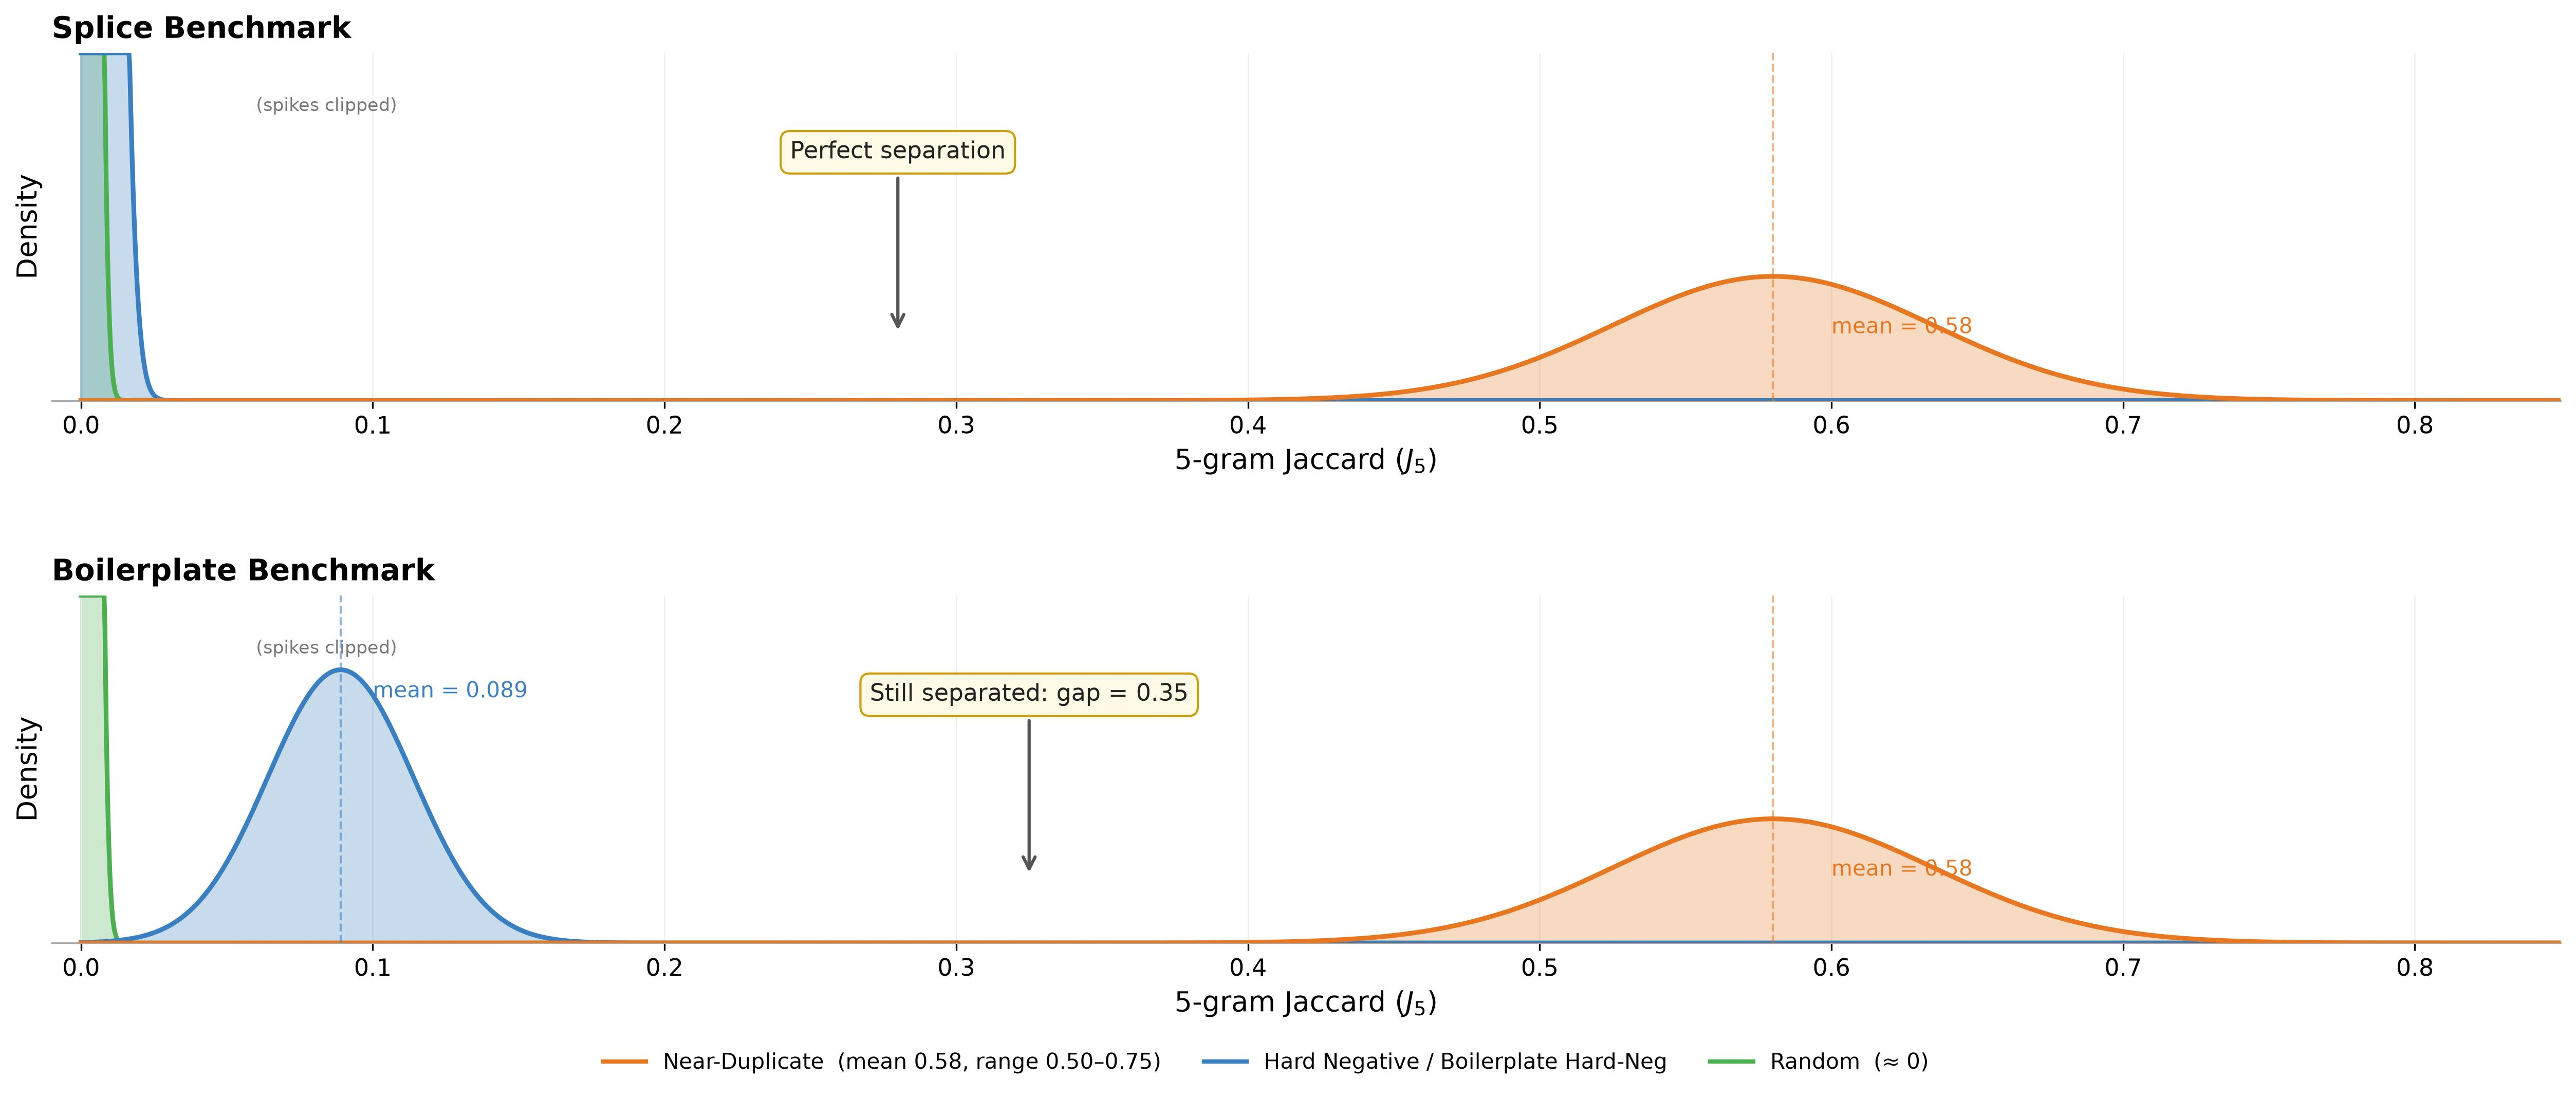
\includegraphics[width=\textwidth,height=0.45\textheight,keepaspectratio]{figures/fig4_v0.jpg}
  \caption{5-gram Jaccard ($J_5$) distributions by pair class on both benchmarks. On the splice benchmark (top), near-duplicate pairs have $J_5 \in [0.50, 0.75]$ (mean 0.58) while both negative classes have $J_5 \approx 0$, creating a perfect separation. On the boilerplate benchmark (bottom), the boilerplate hard-negative class shifts upward to $J_5 = 0.09$--$0.15$ (mean 0.089) due to the shared CC-BY-SA header, but still does not overlap with the near-duplicate range---explaining why Jaccard remains a perfect classifier on this benchmark.}
  \label{fig:fig4}
\end{figure*}

Figure~\ref{fig:fig4} shows the $J_5$ distributions by class on both benchmarks. On the splice benchmark, near-duplicate and hard-negative distributions are entirely non-overlapping. On the boilerplate benchmark, the hard-negative distribution shifts upward (from $J_5 \approx 0$ to $J_5 \approx 0.09$--$0.15$) but still does not overlap with the near-duplicate distribution. The figure makes visible why Jaccard remains a perfect classifier: in neither benchmark does any hard-negative pair reach the near-duplicate Jaccard range.

% ---------------------------------------------------------------
\section{Discussion}
\label{sec:discussion}
% ---------------------------------------------------------------

\subsection{Addressing the Directional Inversion}

The original ecological analogy predicted IoD $\gg 1$ for near-duplicates (local edits = clustered events = high gap variance). This prediction conflates two distinct senses of clustering: (a) \emph{spatial concentration} (edits occur in one region) and (b) \emph{statistical clustering} in the point-process sense (high inter-event gap variance). A single contiguous edit block is the most spatially concentrated arrangement possible, but it produces only a small number of similarly-sized gaps---a nearly degenerate distribution with low variance. The IoD therefore measures the \emph{number and regularity} of edit clusters, not the spatial concentration of a single cluster. Future formulations targeting single-cluster detection should use statistics such as the concentration ratio (\texttt{longest\_run\_frac}) or spatial entropy of the edit density.

\subsection{Why Boilerplate Augmentation Was Insufficient}

The boilerplate benchmark was designed to put hard negatives in the Jaccard range 0.3--0.6, where ECS would need to distinguish distributed overlap (from boilerplate) from localized overlap (from splicing). This required boilerplate of substantial length relative to the article body. The CC-BY-SA license header at $\sim$180 words raised hard-negative $J_5$ to only 0.089--0.15 against articles of 80--800 words. To achieve $J_5 > 0.3$ for hard negatives, the boilerplate would need to constitute more than 30\% of total article length---a regime common in legal documents, terms-of-service pages, and structured templates (e.g., Wikipedia infoboxes), but not reproduced by a short license header alone.

\subsection{When ECS Would Complement Jaccard}

The failure to improve over Jaccard is specific to the experimental constructions. ECS becomes a complementary signal in three concrete scenarios:

\begin{enumerate}
    \item \textbf{Long shared boilerplate.} When legal headers, disclaimers, or structural templates constitute $>$30\% of document length, unrelated documents can reach $J_5 > 0.3$. ECS would correctly identify such pairs as high-IoD (distributed overlap), while splice-based near-duplicates remain low-IoD.

    \item \textbf{Multi-segment edits.} If near-duplicates involve two or more separated edit regions (introduction and conclusion both rewritten), the IoD of those clusters would be higher, converging toward the hard-negative regime. In this scenario, \texttt{longest\_run\_frac} (the fraction of edits in the longest contiguous run) would be a more robust discriminant.

    \item \textbf{Short-shingle regimes.} For character-level unigram or bigram Jaccard on noisy or highly paraphrased text, the Jaccard ceiling breaks. ECS provides an orthogonal structural signal in this regime.
\end{enumerate}

\subsection{Data Consistency Across Iterations}

A discrepancy in the previous paper draft required correction: the cross-validation AUC of 0.973 cited in the prior iteration was computed on synthetic vocabulary-template data (300-word articles generated from 5 topic-specific 60-word vocabularies), not on the Wikipedia benchmark described in the paper. The current experiments run all classifiers on consistent Wikipedia data, yielding a correctly calibrated inverted-ECS AUC of 0.809 $\pm$ 0.025 on the hard subset.

\subsection{Limitations}

\noindent\textbf{Synthetic near-duplicates only.} All near-duplicates are constructed by contiguous splicing. Real-world near-duplication involves multiple separated edits, sentence reordering, word substitution, and paraphrase---patterns with different IoD signatures. The experiment should be replicated on corpora of Wikipedia revision histories or PAN plagiarism detection corpora.

\noindent\textbf{Single domain.} The benchmark draws entirely from Wikipedia, which has consistent article structure, neutral tone, and encyclopedic vocabulary. Results may not generalize to web-crawled text with diverse formatting, legal boilerplate, or domain-specific jargon that constitutes a large fraction of document length.

\noindent\textbf{Small scale.} Nine hundred pairs is sufficient to measure large effects but may underestimate variance in smaller IoD effect sizes. Large-scale evaluation on corpora used in LLM data pipelines (FineWeb \citep{Penedo2024}, RefinedWeb \citep{Penedo2023}) remains future work.

% ---------------------------------------------------------------
\section{Conclusion}
% ---------------------------------------------------------------

We proposed the Edit Clustering Score, a training-free near-duplicate detection feature derived from the Index of Dispersion of inter-edit-gap positions in a word-level LCS diff. The spatial-point-process framing---transplanting IoD from spatial ecology to the 1D sequence of edit positions---is novel in the near-duplicate detection literature. Our corrected main finding is that ECS direction is inverted from the original ecological analogy: contiguous splice-based near-duplicates produce low IoD (one concentrated edit block), while documents sharing scattered coincidental vocabulary produce high IoD (many dispersed edit events). Inverted ECS achieves AUC = 0.81 as a standalone classifier, confirming the discriminative reality of spatial edit structure. ECS does not currently improve over 5-gram Jaccard because splice construction inflates Jaccard perfectly, and our 180-word boilerplate augmentation was insufficient to push hard-negative Jaccard into the ambiguous 0.3--0.6 range.

The clearest path to demonstrating ECS complementarity is a benchmark where boilerplate constitutes $>$30\% of document length (legal or structured content), or a natural revision history corpus where edits are not restricted to single contiguous blocks. We release both benchmarks and all code to support this follow-up work.

\bibliographystyle{plainnat}
\bibliography{references}

\end{document}
